\documentclass{standalone}
\usepackage{tikz}
\usetikzlibrary{arrows.meta}
\begin{document}
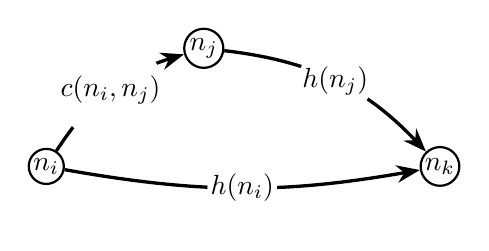
\begin{tikzpicture}
    \draw
    (0,0) node[circle,thick,draw, inner sep=0.6pt](ni){$n_i$}
    (2,1.5) node[circle,thick,draw, inner sep=0.6pt](nj){$n_j$}
    (5,0) node[circle,thick,draw, inner sep=0.6pt](nk){$n_k$}
    ;
    \begin{scope}[
        every node/.style={fill=white,circle, inner sep=0.3pt},
        every edge/.style={-{Stealth[]},draw=black,very thick}]
        \path[->] (ni) edge[bend right=10] node[inner sep=0.1pt] {$h(n_i)$} (nk);
        \path[->] (ni) edge[bend right=-20] node {$c(n_i,n_j)$} (nj);
        \path[->] (nj) edge[bend right=-20] node {$h(n_j)$} (nk);
    \end{scope}
\end{tikzpicture}
\end{document}